\documentclass{article}
\usepackage[T1]{fontenc}
\usepackage{lmodern}
\usepackage{graphicx}
\usepackage{amsmath,amssymb}
\usepackage[a4paper,margin=2cm]{geometry}
\usepackage[absolute,overlay]{textpos}
\setlength{\TPHorizModule}{1mm}
\setlength{\TPVertModule}{1mm}
\usepackage[indonesian]{babel}
\usepackage{hyperref}
\setlength{\emergencystretch}{2em}
% unit: Halaman 51

\begin{document}

% === Halaman 51 (llm) ===

\begin{verbatim}
j = 0;
for (i=0; i<256; i++) {
  j = (j + S[i] + K[i % K.length()]) % 256;
  swap(S[i], S[j]); // Pertukarkan nilai S[i] dan S[j]
}

\vspace{170.48mm}

i = 0; j = 0;
while (!feof(Fin)) {
  p = fgetc(Fin);
  i = (i + 1) % 256;
  j = (j + S[i]) % 256;
  swap(S[i], S[j]); // Pertukarkan nilai S[i] dan S[j]
  t = (S[i] + S[j]) % 256;
  u = S[t]; // keystream
  c = u ^ p;
  fputc(c, Fout);
}
fclose(Fin); fclose(Fout);
\end{verbatim}

% deskripsi: Screenshot potongan kode program dalam bahasa C/C++ yang mengimplementasikan algoritma RC4 (KSA dan PRGA).
% bbox normalisasi: [0.1950, 0.2600, 0.6780, 0.8340]
\begin{textblock*}{101.43mm}(40.95mm,77.22mm)
\noindent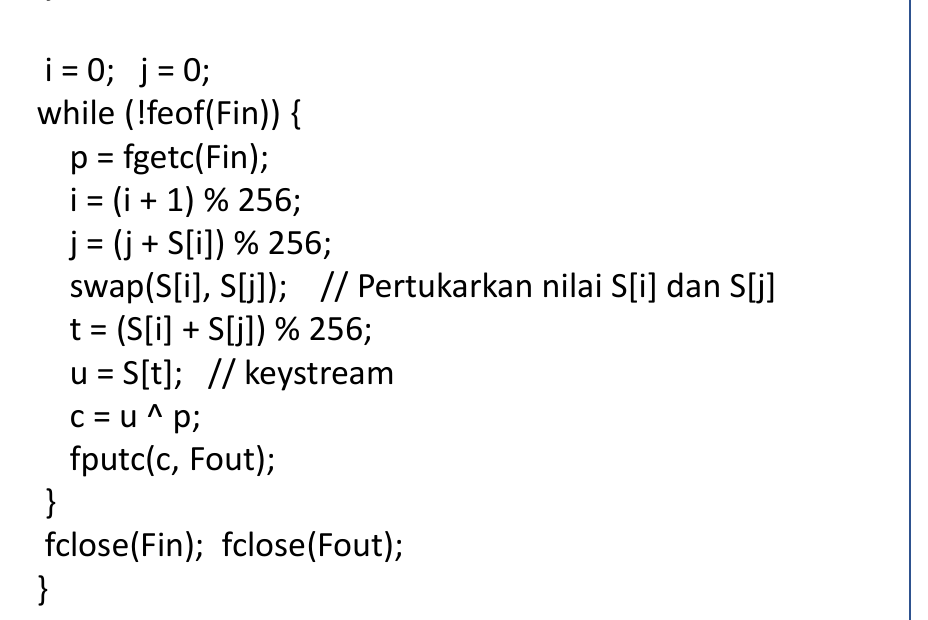
\includegraphics[width=101.43mm,height=170.48mm]{../../images/llm/page_051_img_01.png}%
\end{textblock*}

\end{document}
